\section{Sandwich Theorem}
We can use the Sandwich Theorem to indirectly find limits by "sandwiching" the function in question between two functions we do know the limit of.
If these two sandwiching functions go to the same value in the limit, then so to must the function in question.
\begin{theorem}[The Sandwich Theorem]
	If $g(x) \leq f(x) \leq h(x)$ and $\lim_{x \to c}{g(x)} = \lim_{x\to c}{h(x)} = L$, then $\lim_{x \to c}{f(x)} = L$.
\end{theorem}

\begin{example}
	Evaluate the following limit
	\begin{equation*}
		\lim_{\theta \to 0}{\frac{\sin{\theta}}{\theta}}
	\end{equation*}
\end{example}
We'll need to use some geometric ideas to solve this limit.
Consider the following on a unit circle.

\begin{figure}[H]
	\label{sin_limit_proof}
	\centering
	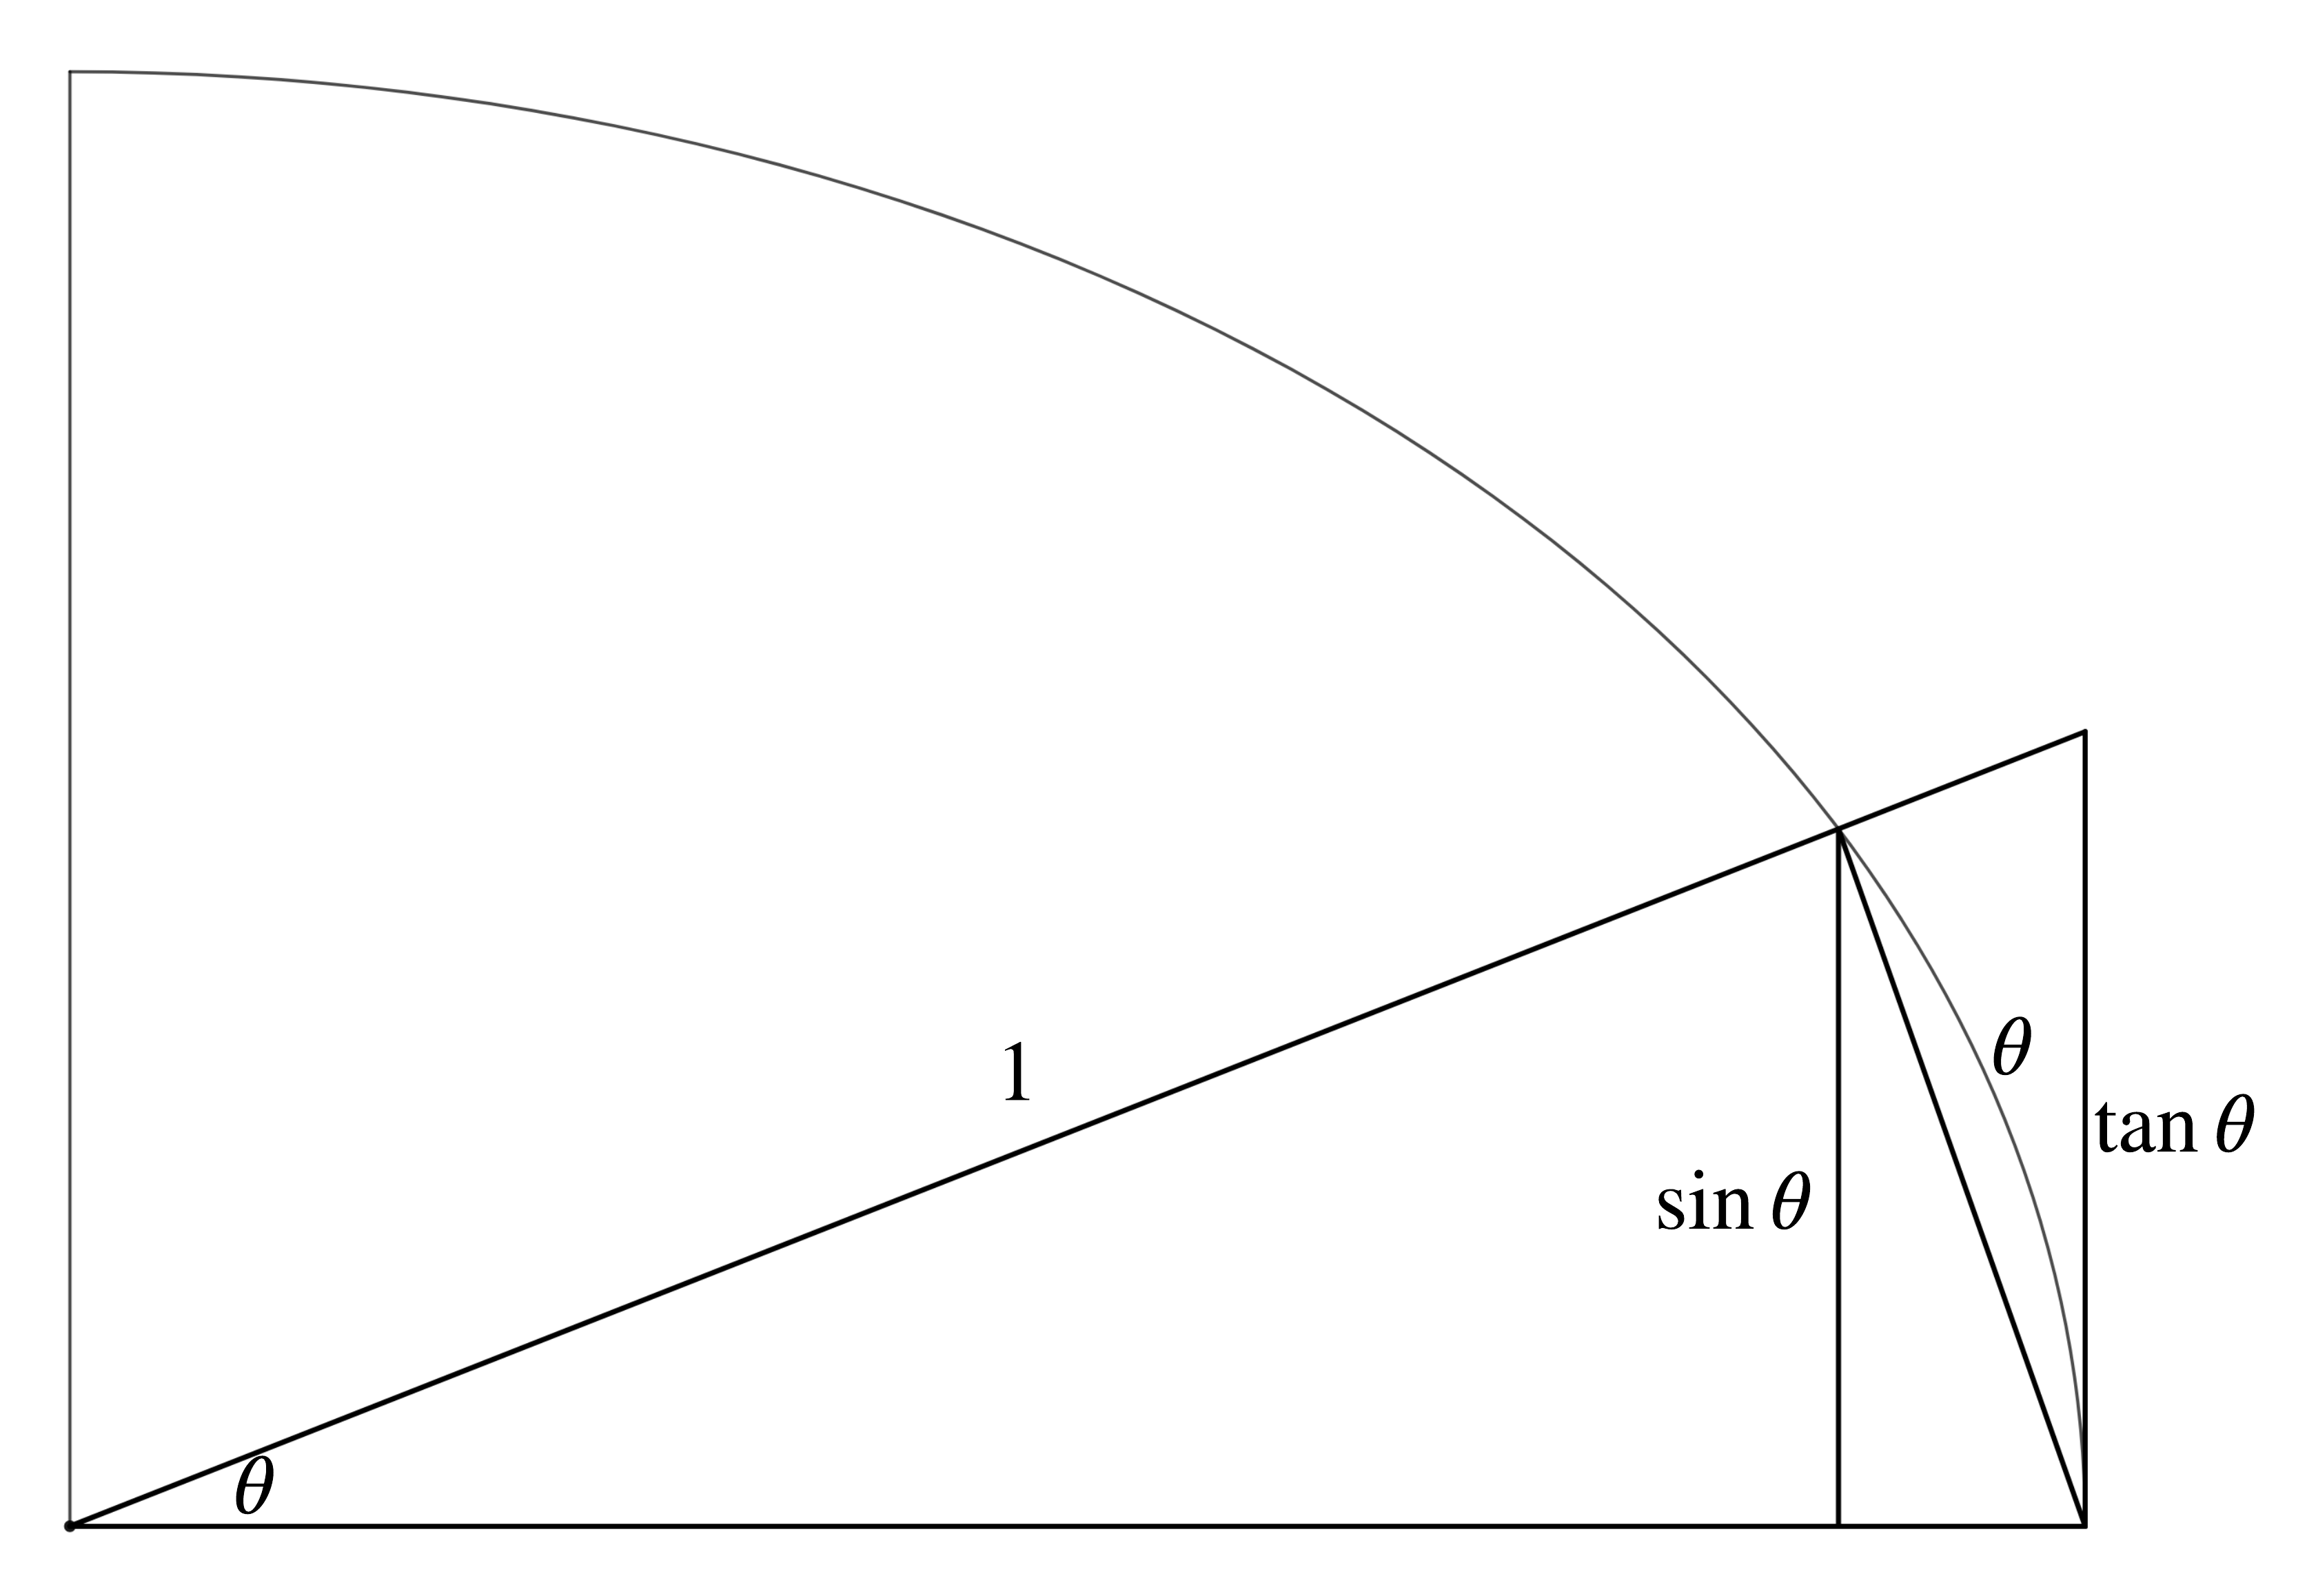
\includegraphics[width = 0.5\textwidth]{./limits_continuity/sin_limit_proof.png}
	\caption{\hyperref{}{}{}{Triangle with internal angle $\theta$ inside a unit circle.}}
\end{figure}

We can see that the area of the swept arc is between the two triangle with base of length 1 and heights of $\sin{\theta}$ and $\tan{\theta}$.
So, we can write the following inequality.
\begin{align*}
	\frac{1}{2}\sin{\theta} &\leq \frac{1}{2}\theta \leq \frac{1}{2}\frac{\sin{\theta}}{\cos{\theta}} \\
	\sin{\theta} \leq \theta &\leq \frac{\sin{\theta}}{\cos{\theta}}
\end{align*}
\indent
Taking the reciprocal of each part and multiplying by $\sin{\theta}$,
\begin{equation*}
	1 \geq \frac{\sin{\theta}}{\theta} \geq \cos{\theta}.
\end{equation*}
\indent
Taking the limit of as $\theta$ approaches 0 of each term,
\begin{align*}
	1 \geq & \lim_{\theta \to 0}{\frac{\sin{\theta}}{\theta}} \geq \lim_{\theta\to 0}{\cos{\theta}} \\
	1 \geq & \lim_{\theta \to 0}{\frac{\sin{\theta}}{\theta}} \geq 1.
\end{align*}
\indent
So, by the Sandwich Theorem,
\begin{equation*}
	\lim_{\theta \to 0}{\frac{\sin{\theta}}{\theta}} = 1.
\end{equation*}